\chapter{Описание методов} \label{ch2}
Данная глава посвящена методам и алгоритмам, используемых в исследовании для обработки и анализа трёхмерных изображений. Глава включает в себя описание разработанных алгоритмов 3D денойзинга и автоматической сегментации флуоресцентных сфер, а также описание уже существующих подходов для предлагаемого решения. 
\section{Описание алгоритма 3D денойзинга} \label{ch2:sec1}
\par В этом параграфе подробно рассмотрены методы шумоподавления двумерных снимков, такие как Non-local Means и Noise2Noise, а также предлагаемое решение в виде комбинации этих методов и их модификации, способное эффективно устранять шум на трёхмерных изображениях с микроскопа.
\subsection{Описание алгоритма NLM (Non-local means)}	
\par Классически существуют два типа моделей по шумоподавлению, а именно локальные и нелокальные. Преимущество первого подхода заключается в его скорости, однако его недостаток состоит в невозможности эффективного сохранения краёв изображений, что проявляется в виде размытия границ и деталей на изображении. Примером локального подхода является Гауссово размытие, а нелокального - метод Non-local means(NLM)\cite{nlm2011}.
%\subsubsection{Размытие по Гауссу}
%\subsubsection{Non-local means}
\par NLM (Non-local means) - это алгоритм для устранения шума на изображении, который обновляет значения пикселей на основе взвешенного среднего значений других пикселей, определённых как наиболее схожие. В отличие от локальных методов, которые используют значения соседних пикселей, NLM использует информацию из всего изображения, что позволяет ему лучше сохранять детали и текстуры. Диаграмма деятельности метода Non-local means приведена ниже на \firef{fig:nlm-schema}.
\par \textbf{Алгоритм метода нелокального среднего (NLM)}\cite{nlm2015}
\begin{enumerate}[]
	\item \textit{Создание окна поиска}:\\
	Создаётся большое окно поиска $S$ размером $K \times K$, центрированное на пикселе $p$. Одновременно создаётся патч(блок пикселей) $N_p$ размером $L$, центрированный на пикселе $p$.
	\item \textit{Вычисление схожести патчей}:\\
	В окне поиска устанавливается новый патч $N_q$, центрированный на пикселе $q$. Затем вычисляется евклидово расстояние $d(p,q)$ между $N_p$ и $N_q$. Далее производится взвешивание патчей с использованием гауссовой функции:
	\begin{equation}
		\tilde w(p,q) = e^{-\frac{d(p,q)}{h^2}}
	\end{equation}
	где $h$ - параметр фильтрации (сглаживания),\\
	$d(p,q) = \|I_y(N_p) - I_y(N_q)\|^2_2$ - евклидово расстояние между $N_p, N_q$\\
	Для наглядности приведен \firef{fig:nlm-weights}, на котором представлена концепция схожести патчей:\\
	\begin{minipage}{\textwidth}
		\centering
		\vspace{\mfloatsep} % интервал  	
		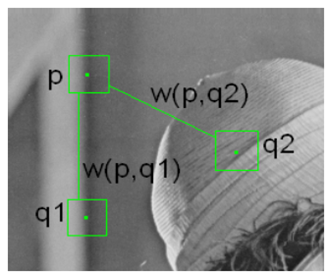
\includegraphics[keepaspectratio=true,scale=0.47] {my_folder/images/denoising/nlm_weights.png}
		\captionof{figure}{Пример,иллюстрирующий концепцию схожестей\\патчей с 3 пикселями: $p, q_1, q_2$ и их весами:\\$w(p, q_1), w(p, q_2)$. $w(p, q_1) > w(p, q_2)$,\\ т.к. патч с $p$ более похож на пачт с $q_1$, чем с $q_2$ }\label{fig:nlm-weights}
		\vspace{\mfloatsep} % интервал  	
	\end{minipage}
	\item \textit{Нормализация весов}:\\
	Проход по всем точкам $q (N_q \in S)$ и нормализация весов:
	 \begin{equation}
		w(p,q) = \frac{\tilde w(p,q)}{\sum_{q \in S} \tilde w(p,q)} 
	\end{equation}
	Согласно формулам, коэффициент веса удовлетворяет условиям:
	\begin{equation}
		\left\{ 
		\begin{array}{ll} 
			\sum_{q} w(p,q) = 1\\
			0 \leq w(p,q) \leq 1 \end{array}\right.
	\end{equation}	
	\item \textit{Вычисление результирующего значения}:\\
	Вычисление результирующего значения обесшумленного пикселя с помощью взвешенной суммы:
	\begin{equation}
		I_z(p) = \sum_{q \in S}w(p,q)I_y(q)
	\end{equation}
\end{enumerate}

\begin{minipage}{\textwidth}
	\centering
	\vspace{\mfloatsep} % интервал  	
	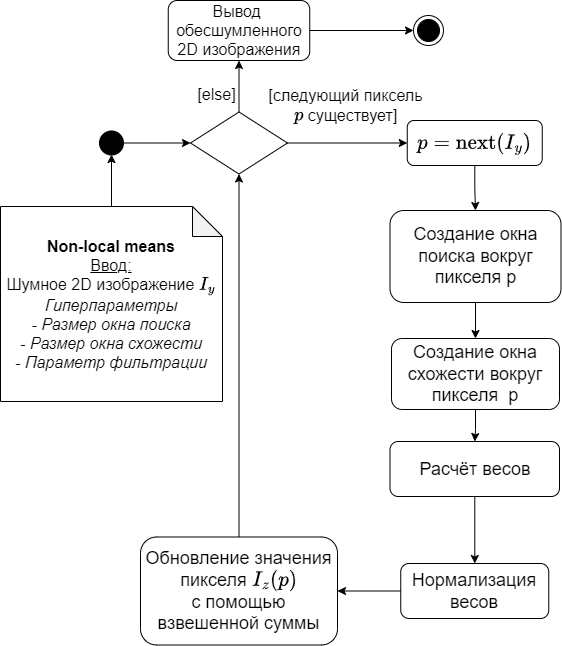
\includegraphics[keepaspectratio=true,scale=0.47] {my_folder/images/denoising/pipeline_nlm_ru.png}
	\captionof{figure}{Диаграмма деятельности Non-local means}\label{fig:nlm-schema}  
	\vspace{\mfloatsep} % интервал  	
\end{minipage}
\subsection{Описание модели Noise2Noise}
\par В качестве метода глубокого обучения была выбрана модель Noise2Noise \cite{noise2noise2018}. Данный подход часто применяется для обработки шумных изображений, таких как флуоресцентные микроскопические снимки с пуассоновско-гауссовым шумом (MPG). В данном описании рассматривается модифицированная версия модели Noise2Noise, включающая дополнительные слои активации, адаптивное обучение и настроенные гиперпараметры. 
\par \textbf{Архитектура сети} изображена на \firef{fig:noise2noise} и представляет собой свёрточную нейронную сеть (CNN), состоящую из энкодера (Encoder) и декодера (Decoder), разбитых на 5 уровней повышения/понижения дискретизации. Каждый уровень состоит из последовательно идущих 2D свёрточных слоёв 3x3, пакетной нормализации, слоя активации Leaky ReLU и соответствующего слоя повышения/понижения дискретизации \cite[с. 337-338]{denoising-imagej-22}. 
\par Из описания архитектуры можно заметить, что данная нейронная сеть является \textit{полносвёрточной}, так как состоит из слоёв свёртки, повышения и понижения дискретизации, активации и пакетной нормализации. Для данной задачи сеть обладает важным свойством - способность обрабатывать входные данные различных размеров. Для данной сети имеется 5 уровней понижения/повышения дискретизации, единственным ограничением на размер входных изображений будет кратность $2^5 = 32$ вдоль всех осей.
\begin{minipage}{\textwidth}
	\centering
	\vspace{\mfloatsep} % интервал  	
	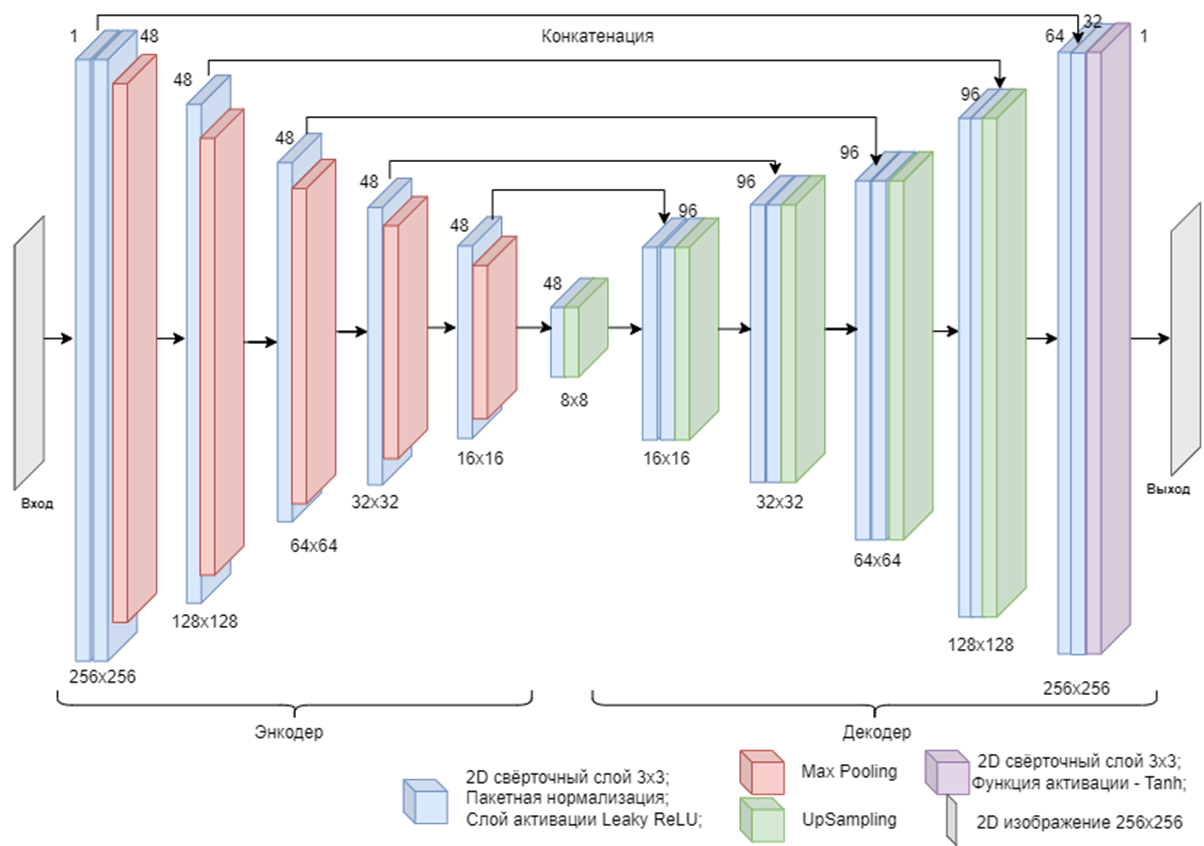
\includegraphics[keepaspectratio=true,scale=0.47] {my_folder/images/denoising/n2n_architecture.png}
	\captionof{figure}{Архитектура сети Noise2Noise}\label{fig:noise2noise}  
	\vspace{\mfloatsep} % интервал  	
\end{minipage}
\par \textbf{Основная идея} Noise2Noise заключается в том, что обучение происходит на паре зашумлённых изображений. Данный факт позволяет сети эффективно удалять шум без необходимости использования чистых изображений в процессе обучения:
\begin{itemize}[]
	\item Вместо использования чистого изображения в качестве цели (label), как это делается в традиционных методах, Noise2Noise использует другое зашумленное изображение того же объекта в качестве цели.
	\begin{equation}
		{I_y}_1 = I_z + N_1,\
		{I_y}_2 = I_z + N_2,\
		\hat I_z = \mathscr{F}_1({I_y}_1)
	\end{equation}
	где $I_z$ - точный сигнал, $N_1, N_2$ - разные шумы, порождающие разные входное и целевое изображения соответственно: ${I_y}_1, {I_y}_2$, $\hat I_z$ - восстановленное изображение, результат $\mathscr{F}_1$.\\
	Поскольку $N_1, N_2$ - случайные величины, они не коррелируют между собой, что позволяет модели учиться выделять общий сигнал $I_z$ присутствующий в обоих изображениях.
	\item Это позволяет модели учиться на данных, где шум разный (например, разные условия съёмки), но сам объект остается неизменным.
	\item Данное свойство делает его особенно полезным в реальных сценариях, где получение чистых данных затруднено или невозможно.
\end{itemize}
\par Данную задачу можно отнести к классу задач с семантическим
разрывом, следовательно, можно выделить класс функций $\mathscr{F}_1(I_y, \theta)$, который позволит найти искомую функцию $\mathscr{F}_1(I_y)$:
\begin{equation}
	\mathscr{F}_1(I_y) = \mathscr{F}_1(I_y, \hat \theta)
\end{equation} где параметр $\hat \theta$ ищется следующим образом:
\begin{equation}
	\hat\theta = \arg\min_{\theta}\mathscr{L}(\hat I_z, {I_y}_2) = \arg\min_{\theta}\mathscr{L}(\mathscr{F}_1(I_y), {I_y}_2)
\end{equation}
где $\theta$ - веса рассматриваемой модели, $\mathscr{L}$ - функция ошибки.\\
В качестве функции потерь $\mathscr{L}$ была взята среднеквадратичная ошибка (MSE), так как она хорошо штрафует за выбросы:\\
\begin{equation}
	MSE(\hat I_z, {I_y}_2) = \frac{1}{N}\sum_{i=1}^{N}(\hat {I_z}_i - {I_y}_{2,i})^2
\end{equation}
где $i = 1..N$ - параметр итерирования по всем точкам изображения, $N$ - общее число точек в изображении.
\par \textbf{Основные модификации модели Noise2Noise}
\begin{itemize}[]
	\item \textit{Нелинейный слой активации (tanh)}:\\
	В исходной архитектуре Noise2Noise используется линейный выходной слой. В модифицированной версии добавлен нелинейный слой активации (tanh) после финального свёрточного слоя. Это помогает лучше моделировать сложные зависимости и улучшает качество денойзинга.\\
	Гиперболический тангенс:
	\begin{equation}
		y_i = \frac{e^{x_i} - e^{-x_i}}{e^{x_i} + e^{-x_i}}
	\end{equation}
	преобразует входное значение в выходное в диапазоне $[-1, 1]$ на $i$-ом слое.
	\item \textit{Адаптивное обучение}:\\ 
	Для ускорения и улучшения процесса обучения используется стратегия адаптивного обучения, известная как \textit{one cycle policy}. Используется линейно-косинусное изменение скорости обучения - сначала происходит линейное увеличение скорости обучения, а затем её косинусное уменьшение.
	\begin{equation}
		\left\{ \begin{aligned} 
			lr(t)= lr_{low} + \frac{t}{start} \times (lr_{max} - lr_{low}), t \leq t_{start},\\
			lr(t)= lr_{end} + \frac{lr_{max} - lr_{end}}{2} \times (\cos(\pi\times t) + 1), t > t_{start}\ldots
		\end{aligned} \right.
	\end{equation}
	$t \in [0, 1]$ - процент выполнения обучения\\
	$t_{start} = 0.3$ - момент перехода от линейного к косинусному изменению\\
	$lr_{max} = 0.0001$ - максимальная скорость обучения\\
	$lr_{low} = \frac{lr_{max}}{25}$ - стартовая скорость обучения, $div = 25$\\
	$lr_{end} = \frac{lr_{max}}{10^4}$ - минимальная скорость обучения\\
\end{itemize}

\subsection{Описание предлагаемого решения}
\par Помимо реализованных алгоритмов денойзинга двухмерных изображений, описанных выше, был разработан алгоритм шумоподавления трёхмерных снимков, комбинирующий в себе оба метода, позволяющий совмещать некоторые достоинства каждого из них.
\par Общая структура предлагаемого алгоритма представлена на \firef{fig:3d-denoise-schema}. Процесс обработки трёхмерных изображений делится на три этапа:
\begin{enumerate}[]
	\item \textit{Предварительная обработка трёхмерного изображения}, включающая следующие шаги:\\
	\begin{enumerate}[]
		\item Перевод изображения в монохром
		\item Z-нормализация
		\begin{equation}
			x_{normalized} = \frac{x-\mu}{\sigma}
		\end{equation}
		где $\mu$ - среднее, $\sigma$ - СКО конкретного слоя
		\item MinMax нормализация
		\begin{equation}
			x_{scaled} = \frac{x - x_{min}}{x - x_{max}}
		\end{equation}
		где $x_{\min}, x_{\max}$ - минимальные максимальные значения всего трёхмерного изображения
	\end{enumerate}
	\item \textit{Основной этап обработки изображения}.\\ Результат предобработки передаётся на вход основному этапу, где пользователь задаёт способ обработки изображений: нелокальный фильтр, нейросетевой подход или их комбинации в различном порядке. Денойзинг производится для каждого слоя независимо друг от друга.
	\item \textit{Склейка слоёв}.\\ На выход подаётся трёхмерное изображение, склеенное из обработанных ранее слоёв.
\end{enumerate}
%\subsubsection{Алгоритм денойзинга трёхмерных снимков}
\begin{minipage}{\textwidth}
	\centering
	\vspace{\mfloatsep} % интервал  	
	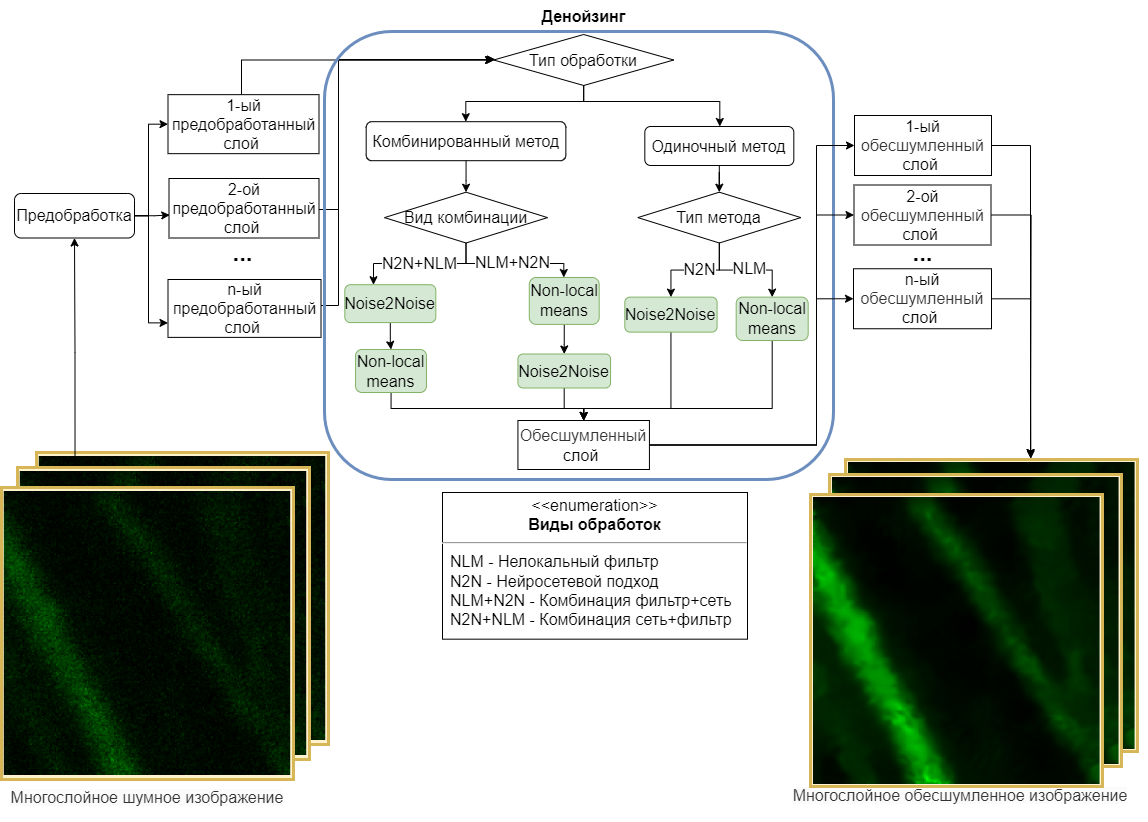
\includegraphics[keepaspectratio=true,scale=0.3] {my_folder/images/denoising/schema_denoising.png}
	\captionof{figure}{Алгоритм 3D денойзинга}\label{fig:3d-denoise-schema}  
	\vspace{\mfloatsep} % интервал  	
\end{minipage}

\section{Описание алгоритма автоматической сегментации флуоресцентных сфер} \label{c2:sec2}
\par Для ускорения процесса ручной сегментации был предложен автоматический подход с использованием методов компьютерного зрения. Для наглядности работы алгоритма продемонстрирована диаграмма деятельности на \firef{fig:autosegm-schema}.
\par \textbf{Алгоритм автоматической сегментации сфер}
\begin{enumerate}
	\item Проведение предварительной обработки
	\begin{enumerate}[]
		\item Перевод изображения в монохром
		\item Применение Гауссова размытия с использованием гиперпараметра радиуса размытия
		\begin{equation}
			G(x,y) = \frac{1}{2\pi\sigma^2}e^{-\frac{x^2+y^2}{2\sigma^2}}
		\end{equation}
		где $x, y$ - координаты точки, $\sigma$ - радиус размытия (стандартное отклонение Гауссового распределения).\\
		Изображение сворачивается с Гауссовым ядром -  каждый пиксель изображения заменяется взвешенной суммой соседних пикселей, где веса определяются значениями Гауссового ядра.
		\item Бинаризация с гиперпараметром порога бинаризации
	\end{enumerate}
	\item Анализ связанных компонент \cite[с. 679-682]{connected-components-2008} - этап, на котором происходит детекция всех сфер (и слипшихся, и одиночных; пример видов сфер на \firef{fig:sphere-types}). Результат анализа - вывод следующих параметров: количество компонент связанности (количество сфер), статистика компонент (координаты границ сфер, объёмы сфер), центроиды (центры сфер).
	\begin{figure}[H]
		\adjustbox{minipage=0.5em,valign=t}{\subcaption{}\label{fig:train-iters-a}}%
		\begin{subfigure}[t]{\dimexpr.5\linewidth-0.5em\relax}
			\centering
			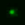
\includegraphics[width=.2\linewidth,valign=t]{my_folder/images/autosegm/good_bead.png}
		\end{subfigure}
		\hfill %выровнять по ширине
		\adjustbox{minipage=0.5em,valign=t}{\subcaption{}\label{fig:train-iters-b}}%
		\begin{subfigure}[t]{\dimexpr.5\linewidth-0.5em\relax}
			\centering
			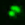
\includegraphics[width=.2\linewidth,valign=t]{my_folder/images/autosegm/bad_bead.png}
		\end{subfigure}
		\\[20pt]
		\captionsetup{justification=centering} %центрировать
		\caption{Виды сфер в результате анализа связанных компонент: {\itshape a} --- одиночная сфера; {\itshape b} --- слипшиеся сферы} 
		\label{fig:sphere-types}
	\end{figure}
	\item Фильтрация сфер на основе предложенного объёма правильной (одиночной) сферы. Если объём конкретной сферы меньше заданного, то она распознаётся как правильная и сохраняется.
	\item Извлечение трёхмерных сфер с заданным гиперпараметром ограничивающего прямоугольника.
	\item Усреднение флуоресцентных сфер. Считается выборочное среднее по всем извлечённым.  
	\item Вывод результатов (усреднённой сферы и снимка с сегментированными сферами).
\end{enumerate}
\begin{minipage}{\textwidth}
	\centering
	\vspace{\mfloatsep} % интервал  	
	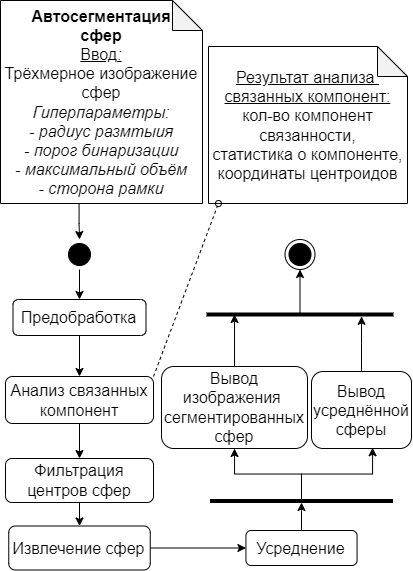
\includegraphics[keepaspectratio=true,scale=0.4] {my_folder/images/autosegm/schema.png}
	\captionof{figure}{Диагрпамма деятельности автоматической сегментации сфер}\label{fig:autosegm-schema}  
	\vspace{\mfloatsep} % интервал  	
\end{minipage}
\textbf{Замечание}
\par Значения гиперпараметров подбирались экспериментальным  способом. Благодаря быстрой работе методов и заданным значениям по умолчанию, у человека есть возможность менять показатели в реальном времени, отслеживая динамику работы.
